\section{The model}
\label{sec:the-model}
In this section we will go through the model from the article \cite{self-org} 
in great detail. 
 
As mentioned earlier in section~\ref{subsec:ABapproach} the social force model 
is an agent based model, this means that we describe the system by looking at 
each individual object of the system. In this case each object in the system 
is subject to a series of social forces. These forces are not real physical 
forces in the sence that they follow newtons laws of motion but rather a 
measure of the agents motivation for acting in specific ways. However that 
name \emph{social forces} is not accidential, we borrow both notation and to 
some extent the interpretation from physics. In the model we are studying 
there are four different forces. They are \emph{the desired force}, \emph{the 
repulsive force from walls}, \emph{the interaction force} and \emph{the 
attractive force}. All the forces work in the horizontal plane, the vertical 
plane is not of interest. The forces are illustrated in 
figure~\ref{ForceModel}.  They will all be studied closely in turn in the 
following sections.

\begin{figure}[hb]
    \centering
    {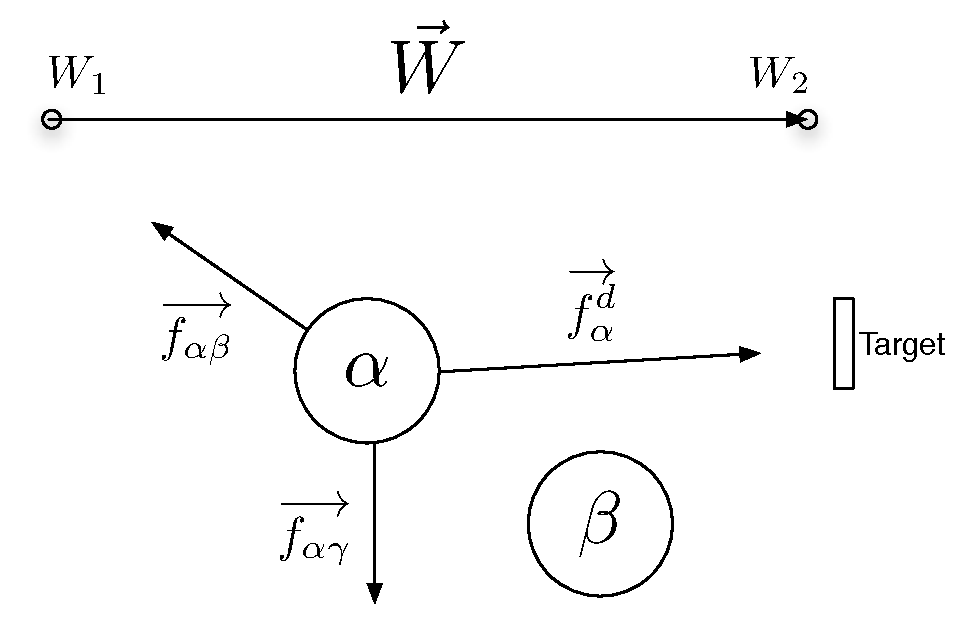
\includegraphics[scale=0.45]{Figures/ForceModel.pdf}} \caption[Notation 
    of forces acting on an agent]{Illustration of the forces acting on an 
    agent $\alpha $. $ \beta $ is another agent and the grey bar on the top 
    represents a wall. $ \vec{f_{\alpha\beta}} $ is the repulsive force from 
    agent $ \beta $, and $ \vec{f_{\alpha B}} $ is the repulsive force from 
    the wall. $ \vec{f^{0}_{\alpha}} $ is a force that represents agent $ 
    \alpha $'s desire to reach the exit.  The x and y axes are defined by the 
    Cartesian coordinate system.}
    \label{ForceModel}
\end{figure}

\subsection{The equation of motion for agent $ \alpha $:}
The purpose of the model is to describe how each agent moves so an equation of 
motion for each agent is needed. They way to get this equation of motion is 
much like one would in physics by summing up akk the forces acting on the 
agent. This gives rice to an acceleration of the agent and from this one is 
able to derive the exact movement of the agent. Again it is important that 
this is a method borrowed from physics, we are not working with real physical 
forces here.

Each induvidual agent is has a series of parameters describing the features of 
the agent. An agent is represented by a circle with radius $r_{\alpha}$. The 
agent has a position $\vec{r_{\alpha}}$ and a velocity $\vec{V_{\alpha}}$ at 
all times t. Furthermore each agent has a desired direction $\vec{e_{\alpha}}$ 
in which it would like to go. An illustration of the notation can be seen in 
figure \ref{fig:NotationOfAgent}.

\begin{figure}[hb]
    \centering
    {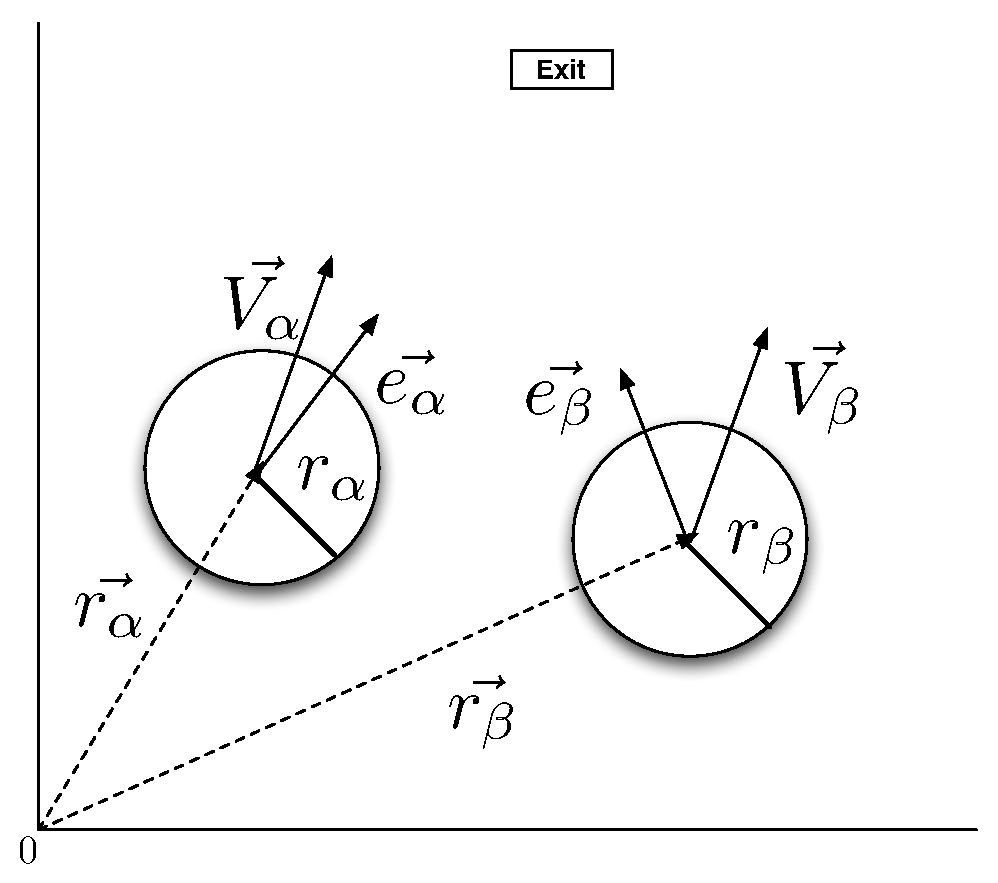
\includegraphics[scale=0.35]{Figures/NotationOfAgent.pdf}} 
    \caption[Notation of an agent]{Illustration of the visual presentation of 
    the mathematical notations for position and velocity. As for agent $ 
    \alpha $, it has position vector $ \vec{r_{\alpha}} $, velocity vector $ 
    \vec{V_{\alpha}} $, $\vec{e_{\alpha}}$ or $\vec{e_{\beta}}$ the normal 
    vector pointing to the exit and  $ r_{\alpha} $ or  $ r_{\beta} $ the 
    radius of its body.  The x and y axes are defined by the Cartesian 
    coordinate system.}
    \label{fig:NotationOfAgent}
\end{figure}

The change in position $ \vec{r_{\alpha}} $ per time of agent $\alpha$ is the 
velocity $ \vec{V_{\alpha}} $:

\begin{equation}
		\frac{d \vec{r_{\alpha}}}{dt} = \vec{V_{\alpha}} \left( t \right)
\end{equation}

The change of velocity per time is the acceleration of agent $\alpha$, which 
is due to all the forces acting on the agent. The summation of all the forces 
is called $\vec{f_{\alpha}} \left( t \right)$ and it is given by:

\begin{equation}
    \frac{d \vec{V_{\alpha}}}{dt} = \vec{f_{\alpha}} \left( t \right) 
\end{equation}

The summation of all the forces can be devided into four terms as stated in 
the introduction to this section.

\begin{equation}\label{model}
    \vec{f_{\alpha}} = \vec{f^{0}_{\alpha}} + \vec{f_{\alpha B}} +
    \sum_{\beta \neq \alpha} \vec{f_{\alpha \beta}} +  
    \sum_{i} \vec{f_{\alpha i}} 
\end{equation}

Here $\vec{f_{\alpha}^{0}}$ is the \emph{desired force}, $\vec{f_{\alpha 
\text{B}}}$ is the repulsive force from walls. $\vec{f_{\beta \neq \alpha}}$ 
is a repulsive force from other agents and $\vec{f_{\alpha i}}$ is a 
attractive force.

We will now move on to show the explicit expression for each force. We will go 
through them one at a time explaining their mathematical structure and their 
role in the model.

\subsection{The desired force}
The first term on the right hand side of equation \eqref{model} describes the 
\emph{willingness} of agent $\alpha$'s to reach the exit. It is a velocity 
dependent force and is given by:

\begin{equation}\label{relaxtime}
	\vec{f^{0}_{\alpha}}\left( \vec{V_{\alpha}} \right) =
    \frac{1}{\tau}
    \left( V_{\alpha}^{0} \vec{e_{\alpha}} - \vec{V_{\alpha}} \right)
\end{equation}

Where $V_{\alpha}^{0}$ is the desired speed, $ \vec{e_{\alpha}} $ is the unit 
vector pointing in the desired direction of the agent which in most cases will 
be the exit, but it can in principle be anywhere.  $\vec{V_{\alpha}}$ is the 
actual velocity of the agent, and $\tau$ is the \emph{relaxation time}.

The relaxtion time determines how reactive a agent is. In principle the 
relaxation time can vary for each agent but from the article \cite{self-org} 
we get that $ \tau_{\alpha}\approx 1s $, which means that it takes the agent $ 
1s $ to change its velocity. $V_{\alpha}^{0} \vec{e_{\alpha}}$ is the desired 
velocity of the agent. The desired speed at some time $V_{\alpha}^{0}\left( t 
\right)$ is given by:

%TODO: Write a section about the notation
% About the notation, any quantity with a "$ ^{0} $ " on the upper right corner 
% is a "desired" quantity.


\begin{equation}\label{v0eta}
    V_{\alpha}^{0}\left( t \right) = \left[ 1 - \eta_{\alpha} \left( t \right) \right] 
    V_{\alpha}^{0} \left( 0 \right) +
    \eta_{\alpha} \left( t \right)V_{\alpha}^{\text{max}}
\end{equation}

where $V_{\alpha}^{0} \left( 0 \right)$ is the desired speed at $ t=0 $, and 
$V_{\alpha}^{\text{max}}$ is the maximum desired speed of agent $\alpha$. The 
maximum desired speed is the speed that agent $\alpha$ will try to get if it 
is allowed by the environment and other agents. It is not a physical limit to 
how fast the agent can move but rather a parameter that determines the speed 
that the agent is comfortable walking with. 

The desired speed $V_{\alpha}^{0} \left( t \right)$ Changes with time, and 
especially varies with the impatience factor which is also a function of time 
$t$.

$\eta_{\alpha}$ is called the impatience or nervousness of the agent and is 
given by:

\begin{equation}\label{eta}
	\eta_{\alpha} \left( t \right) =
    1 - \frac{\overline{V}_{\alpha} \left( t \right)}
             {V_{\alpha}^{0} \left( 0 \right)}
\end{equation}

where $\overline{V}_{\alpha}\left( t \right)$ is the average speed in the 
desired direction.Excately how one measures the average speed in the desired 
direction is not properly explained in the article. We define it to be the 
projection of the position vector $ \vec{r_{\alpha}} $ onto the desired direction 
of motion $e_{\alpha}$ devided by the time that the simulation has run. A 
illustration of this can be seen i figure \ref{impatience}. The mathematical 
expression becomes:


\begin{figure}[ht]
    \centering
    {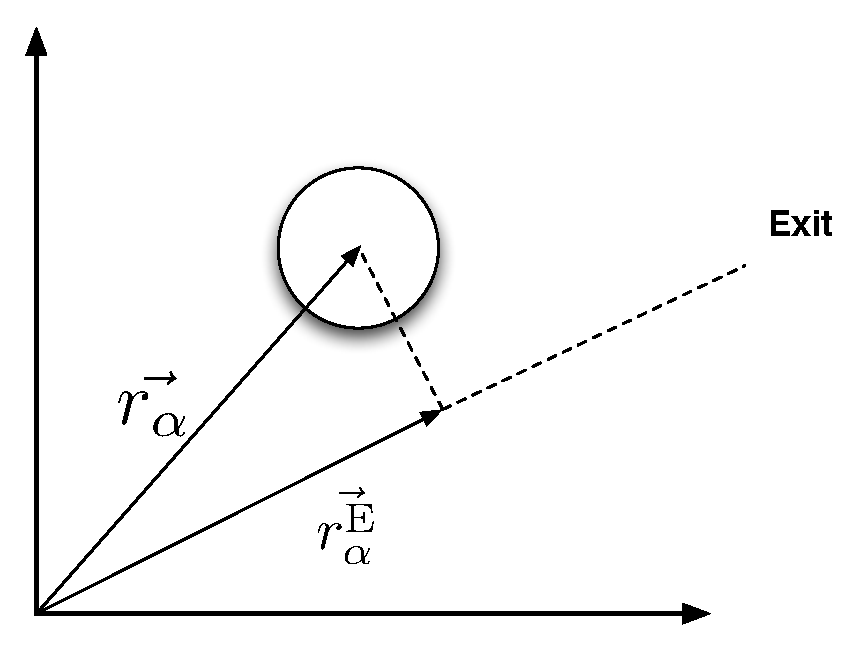
\includegraphics[scale=0.35]{Figures/NotationOfAgent2.pdf}} 
    \caption{Illustration of the vector $ \vec{r_{\alpha}^{E}}$, which is the 
    projection of $ \vec{r_{\alpha}} $ onto the desired direction of motion.}
    \label{impatience}
\end{figure}

\begin{equation}\label{averagespeed}
   \overline{V}_{\alpha} \left( t \right) =
   \frac{1}{t} \vec{r_{\alpha}}\cdot \vec{e_{\alpha}} 
\end{equation}

$\overline{V}_{\alpha}$ is undefined at $t=0$ beacause that would mean 
that you should devide by zero, which is undefined. This in turn means 
that $\eta_{\alpha}(0)$ is undefined. We therefore define 
$V_{\alpha}^{0}(t)$ for $t=0$ and $t>0$ to be the following:

\[
  V_{\alpha}^{0} (t) = \left\{ 
  \begin{array}{l l}
    V_{\alpha}^{0}(0) \quad \text{if $t=0$}\\
    \left[ 1 - \eta_{\alpha} \left( t \right) \right] 
    V_{\alpha}^{0} \left( 0 \right) +
    \eta_{\alpha} \left( t \right)V_{\alpha}^{\text{max}} \quad \text{if $t>0$}\\
  \end{array} \right.
\]

%\begin{eqnarray}
%    \eta_{\alpha} \left( 0 \right) &=&
%    1 - \frac{\overline{V}_{\alpha} \left( 0 \right)}
%    {V_{\alpha}^{0} \left( 0 \right)}\\
%    &=& 1 - \frac{0}{V_{\alpha}^{0} \left( 0 \right)}
%    = 1
%\end{eqnarray}
%
%which makes sense, as when the emergency suddenly happens our agent should 
%feel extremely anxious ($ \eta_{\alpha} \left( 0 \right)=1 $). Then we know 
%the initial desired speed $ V_{\alpha}^{0}\left( 0 \right) $ is
%
% \begin{equation}
%     \begin{split}
%         V_{\alpha}^{0}\left( 0 \right) &= 
%             \left[ 1 - \eta_{\alpha} \left( 0 \right) \right] 
%             V_{\alpha}^{0} \left( 0 \right) +
%             \eta_{\alpha} \left( 0 \right)V_{\alpha}^{\text{max}}\\
%         &= \left( 1 - 1 \right)  
%             V_{\alpha}^{0} \left( 0 \right) +
%             1 V_{\alpha}^{\text{max}}\\
%         &= V_{\alpha}^{\text{max}}
%     \end{split}
% \end{equation}
% 
% Equation (\ref{v0eta}) and Equation (\ref{eta}) contains an intermediate 
% variable $ \eta_{\alpha} \left( t \right) $, so in principle we are allowed to 
% eliminate $ \eta_{\alpha} \left( t \right) $ and only show the relationship 
% between $ V_{\alpha}^{0}(t) $ and $ \overline{V}_{\alpha} \left( t \right) $. 
% Thus we get:
% 
% \begin{equation}\label{vv}
%     V_{\alpha}^{0}(t) =
%         \left[ 
%             1 - \frac{V_{\alpha}^{max}}{V_{\alpha}^{0}(0)}
%         \right] \overline{V}_{\alpha} \left( t \right) +
%         V_{\alpha}^{max}
% \end{equation}
% 
% \begin{figure}[ht]
%     \centering
%     {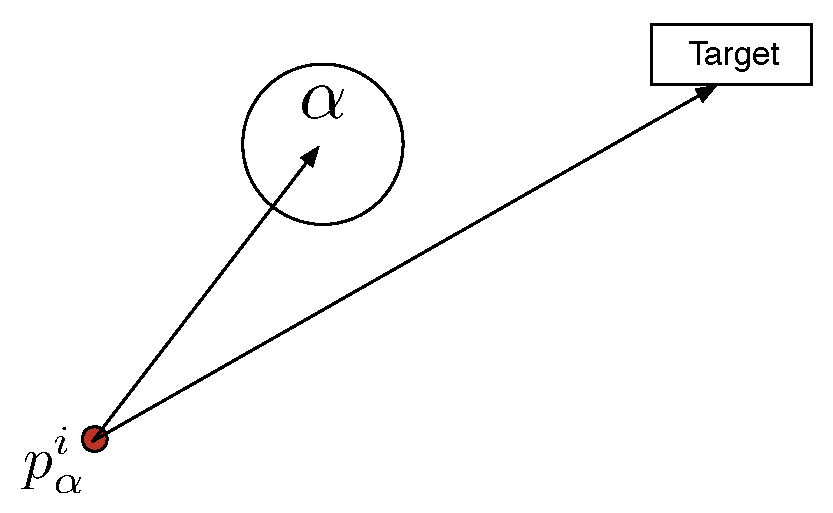
\includegraphics[scale=0.35]{Figures/impatience.pdf}} \caption[The 
%     impatience factor]{Illustration on the correlation between the function 
%     about the desired speed $ V_{\alpha}^{0}(t) $ and the average speed in the 
%     desired direction of motion $ \overline{V}_{\alpha} \left( t \right) $, 
%     and the graph of $ V_{\alpha}^{0}(t) = \left[ 1 -  
%     \frac{V_{\alpha}^{max}}{V_{\alpha}^{0}(0)}\right] \overline{V}_{\alpha} 
%     \left( t \right) + V_{\alpha}^{max} $ intersects with the axis at $ \left( 
%     0 , V_{\alpha}^{max} \right)  $ and $ \left(V_{\alpha}^{max} 
%     \frac{V_{\alpha}^{0} \left( 0 \right) }{V_{\alpha}^{max}-V_{\alpha}^{0} 
%     \left(0 \right)} , 0 \right)  $.  When $\alpha$'s velocity is at maximum 
%     the impatience gets low, and vice versa.}
%     \label{fig:impatience}
% \end{figure}
% 
% Figure (\ref{fig:impatience}) is a drawing of the graph about those two 
% variables, and the intersection of the function line with both axis are:
% 
% \begin{equation}
%     \left( 
%         \overline{V_{\alpha}} , V_{\alpha}^{0} \left( t \right)
%     \right)
%     =
%     \left( 
%         0 , V_{\alpha}^{max} 
%     \right) 
%     \text{and} 
%     \left(
%         V_{\alpha}^{max} 
%         \frac
%             {V_{\alpha}^{0} \left( 0 \right) }
%             {V_{\alpha}^{max}-V_{\alpha}^{0} \left(0 \right)} 
%         , 0 
%     \right) 
% \end{equation}
% 
% Normally, the values of the two speeds should have positive values, so the 
% graph is part of a straight line.Now there is a doubt the range of the value 
% of $ \overline{V}_{\alpha} \left( t \right) $, compared with $ 
% V_{\alpha}^{max} $, if we have already set $ V_{\alpha}^{max} $ a fixed number 
% for a certain agent. In the case:
% 
% \begin{equation}
% 	V_{\alpha}^{max} 
% 	\geq 
% 	V_{\alpha}^{max} 
% 	\frac{V_{\alpha}^{0}(0)}{V_{\alpha}^{max}-V_{\alpha}^{0}(0)}
% \end{equation}
% 
% we get the relation:
% 
% \begin{equation}
%     V_{\alpha}^{0}(0)\leq \frac{1}{2} V_{\alpha}^{\text{max}}
% \end{equation}
% 
% Which contradicts with our earlier conclusion that
% 
% \begin{equation}
%     V_{\alpha}^{0}\left( 0 \right) = V_{\alpha}^{\text{max}}
% \end{equation}
% 
% Therefore, the graph should not intersect with $ \overline{V_{\alpha}} $ axis 
% under normal circumstances when the maximum desired velocity is not exceeded.
% However, from Equation \ref{vv}  and Figure \ref{impatience} we think that 
% $V_{\alpha}^{\text{max}}$ can be exceeded, but only under rare situations. For 
% example, at $ t=0 $, if agent $ \alpha $ moves opposite to the exit because of 
% some extreme large repulsive force, then from Equation \ref{vv} $ 
% V_{\alpha}^{0} \left( 0 \right)  $ is larger than $V_{\alpha}^{\text{max}}$.
% 
% If there are no repulsive forces at all, the only source of acceleration is 
% from the desired velocity, which modifies the actual velocity to the desired 
% direction and value.  After some time, the actual velocity should reach some 
% constant, which resembles the so called terminal velocity in physics when the 
% acceleration is zero.  When the agent reaches the terminal velocity the actual 
% velocity does not change and it equals the average velocity, so we can write 
% the acceleration from Equation \ref{relaxtime} as
% 
% \begin{equation}
%     \vec{f}_{\alpha} = \vec{f^{0}_{\alpha}}\left( \vec{V_{\alpha}} \right)
% \end{equation}
% 
% \begin{equation}
%     \frac{1}{\tau}
%     \left( 
%         V_{\alpha}^{0} \vec{e_{\alpha}} - 
%         \overline{V}_{\alpha} \left( t \right) \vec{e_{\alpha}}  
%     \right)  = 0
% \end{equation}
% 
% As $ \tau $ is a constant, despite the direction of the velocity vector we have:
% 
% \begin{equation}\label{terminal}
% 	 V_{\alpha}^{0} - \overline{V}_{\alpha} \left( t\right) = 0
% \end{equation}
% 
% Also we take Equation \ref{vv}, and insert the value of $ V_{\alpha}^{0}(t) $ 
% from Equation \ref{vv} to Equation \ref{terminal}:
% 
% \begin{equation}
% 	\left[ 
%         \left(
%             1 - \frac{V_{\alpha}^{max}}{V_{\alpha}^{0}(0)}
%         \right)
%         \overline{V}_{\alpha} \left( t \right) + V_{\alpha}^{max} 
%     \right] - \overline{V}_{\alpha} \left( t\right) 
%     = 0
% \end{equation}
% 
% Solve for $ \overline{V}_{\alpha} \left( t\right) $ we get:
% 
% \begin{equation}
%     \overline{V}_{\alpha} \left( t\right) = V_{\alpha}^{0}(0)
% \end{equation}
% 
% Which makes a lot of sense because the terminal velocity is the initial 
% desired velocity and equals the maximum desired velocity.
% 
% The impatience or nervousness factor is active when one calculates the force 
% action on agent $\alpha$ from the velocity of the agent.

If we look at the expression for $V_{\alpha}^{0}$ for $t>0$ we can 
start to analyse how this affects the behavior of the agent. There 
are three cases that is of interestes, namely $0 < \eta_{\alpha} < 1$, 
$\eta_{\alpha} < 0$ and $1 < \eta_{\alpha} $.

In the case where $0 \leq \eta_{\alpha} \leq 1$ the expression for 
$V_{\alpha}^{0} \left( t \right)$ makes sense. Here we can see why this term 
is called the impatience of the agent. If the fraction  between the average 
speed in the desired direction and the initial desired speed is low then 
$\eta_{\alpha} \approx 1$. 
When the impatience term is close to one $V_{\alpha}^{0} \left( t \right)$ is 
dominated by $V_{\alpha}^{\text{max}}$. That is, if the agent have not moved 
very far in the desired direction compared to the initial speed the impatience 
of the agent will cause the agent's future velocity to be dominated by the 
desired velocity of the agent. 
If the agent has been moving in the desired direction with his initial speed 
the entire time then $\eta_{\alpha} = 0$  and $V_{\alpha}^{0} \left( t 
\right)$ will continue to be $V_{\alpha}^{0} \left( 0 \right)$. 

However in the case where $\eta_{\alpha} < 0$, that is the agent has moved 
further in the desired direction than he would have had he been walking with his 
initial speed. This can happen in situations where then agent is being pushed 
forward forward by the crowd.

In the case where $1 < \eta_{\alpha}$ that is the agent has moved further 
in the opposite direction than the desired one. Then can happen if the agent 
starts out by being very close to another agent. However this is not something 
that we think will happen very often. In any circumstances it will only have an 
effect very early in the simulation. 

This concludes the explanation of the first of the four physical forces. The next 
force in the equation is the repulsive force from the walls.

\subsection{Repulsion from the walls}
The second term on the right hand side of equation \eqref{model} is a force which arise from interactions with the walls or other obstacles. The forces, caused by the wall or obstacles, is given by:

\begin{equation}\label{wallpotential}
    \vec{f_{\alpha B}} \left( \vec{r_{\alpha}} \right) =
    - \nabla_{\vec{r_{\alpha}}} U_{B}
    \left( \| \vec{r_{\alpha}} - \vec{r_{B}^{\alpha}} \| \right)
\end{equation}
$U_B$ is a repulsive potential and $ \| \vec{r_{\alpha}} - \vec{r_{B}^{\alpha}} \|$ is the distance 
from the position of agent $\alpha$ to the nearest point $ \vec{r_{B}^{\alpha}}  $ of the wall and shown in figure \ref{NotationOfWall}.

\begin{figure}[ht]
\centering
{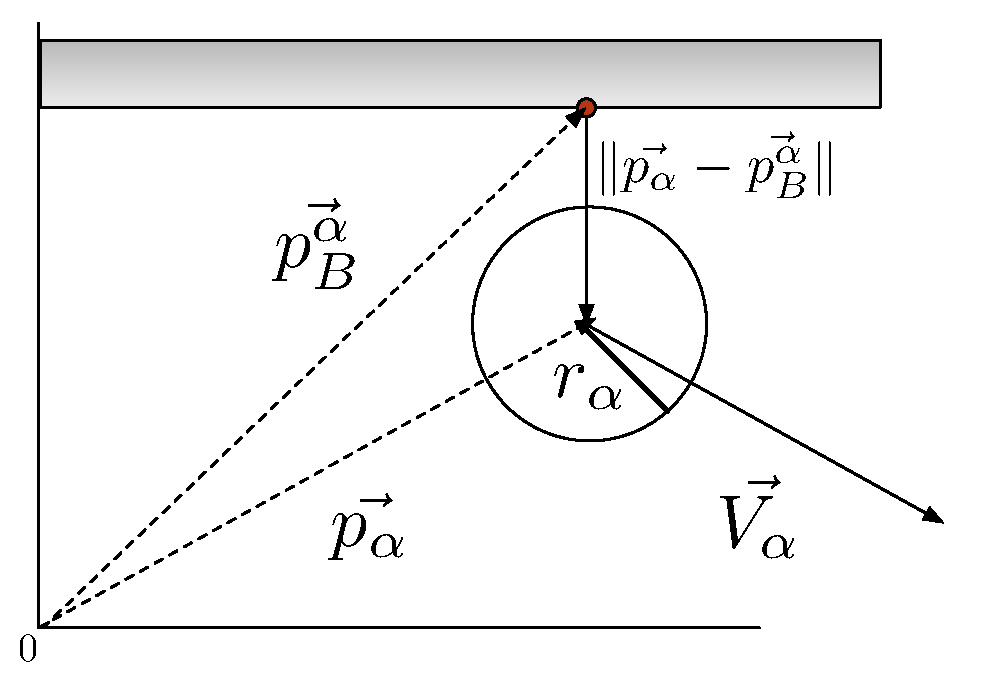
\includegraphics[scale=0.35]{Figures/NotationOfWall.pdf}} 
\caption[Notation of the interaction between an agent and a wall]{The illustration shows the mathematical notation for the interaction with walls used. The circle is pedestrian $\alpha$ with radius $r_{\alpha}$, $\vec{r_{\alpha}}$ is the position vector for $\alpha$, the grey box on the top is the wall, $\vec{r_{B}^{\alpha}}$ is the position vector for the closest part of the wall to $\alpha$, $\left( \| \vec{r_{\alpha}} - \vec{r_{B}^{\alpha}} \| \right)$ is the smallest distance from $\alpha$ to the wall and $\vec{V_{\alpha}}$ is the velocity vector for $\alpha$.}
\label{NotationOfWall}
\end{figure}

\begin{itemize}
\item  $U_B$ only depends on the distance $ \| \vec{r_{\alpha}} - \vec{r_{B}^{\alpha}} \|$, so the gradient of $V_B$ tells us in which direction does this distance change the most. It is obvious that the changes is largest if the agent takes a step directly towards or away from the wall, which means that the agent will always be pushed directly away from the wall.

\item The next job is to find an explicit expression for $ \| \vec{r_{\alpha}} - \vec{r_{B}^{\alpha}} \|$\\
To start of with we need to find point on the wall that is perpendicular to $\alpha$ as it will be the nearest.  
If we define the wall as a vector, $\vec{W}$ going from a point in space $w_1$ to another point $w_2$, then we can find the projection of $\alpha$ onto the wall and this projection will be $\vec{r_{B}^{\alpha}}$.
The equation for the projection is
\begin{equation}\label{wall}
\vec{r_{B}^{\alpha}}=\frac{\vec{r_{\alpha}}\cdot \vec{W}}{\| \vec{W} \|^2}\vec{W}
\end{equation}
With this we now have the two points we need to calculate $ \| \vec{r_{\alpha}} - \vec{r_{B}^{\alpha}} \|$.


\item With the explicit expression for $ \| \vec{r_{\alpha}} - \vec{r_{B}^{\alpha}} \| $, we are able to calculate $ \vec{f_{\alpha B}} \left( \vec{r_{\alpha}} \right) $ from Equation \ref{wallpotential}, if the expression for the potential function $ V_{B}
    \left( \| \vec{r_{\alpha}} - \vec{r_{B}^{\alpha}} \| \right) $ is given.\\
In some of the other articles [ ] made by the same outhers as the article which makes the basis for the model in this repport, the repulsive potential from the wall is given as
\begin{equation}
U_{B} \left( \| \vec{r_{\alpha}} - \vec{r_{B}^{\alpha}} \| \right) =
U^0_{\alpha B} e^{- \| \vec{r_{\alpha}} - \vec{r_{B}^{\alpha}} \| / r_{\alpha} }
\end{equation}
where $U^0_{\alpha B}$ is a constant and $r_{\alpha}$ is the radius of a pedestrian $\alpha$. \\

In that case, the repulsive force on agent $ \alpha $ from the wall is:
\begin{equation}
    \vec{f_{\alpha B}} \left( \vec{r_{\alpha}} \right) =
    - \nabla_{\vec{r_{\alpha}}} U_{B}
    \left( \| \vec{r_{\alpha}} - \vec{r_{B}^{\alpha}} \| \right)\\
=-\left( \frac{\partial}{\partial x_{\alpha}}U_{B}( \| \vec{r_{\alpha}} - \vec{r_{B}^{\alpha}} \|), \frac{\partial}{\partial y_{\alpha}}U_{B}( \| \vec{r_{\alpha}} - \vec{r_{B}^{\alpha}} \|)\right) \\
\end{equation}
Calculating the derivatives we use that $\| \vec{r_{\alpha}} - \vec{r_{B}^{\alpha}} \|= \sqrt{(x_{\alpha}-x^{\alpha}_{B})^2+(y_{\alpha}-y^{\alpha}_B)^2}$.
Inserting this and the expression for $U_{B}$ we get:

\begin{equation}
\begin{split}
\vec{f_{\alpha B}} \left( \vec{r_{\alpha}} \right) 
& =-\left( \frac{\partial}{\partial x_{\alpha}}U^0_{\alpha B} e^{-\sqrt{(x_{\alpha}-x^{\alpha}_{B})^2+(y_{\alpha}-y^{\alpha}_B)^2}/r_{\alpha} }\right. , \\
& \left. \frac{\partial}{\partial y_{\alpha}}U^0_{\alpha B} e^{-\sqrt{(x_{\alpha}-x^{\alpha}_{B})^2+(y_{\alpha}-y^{\alpha}_B)^2}/r_{\alpha} } \right)
\end{split}
\end{equation}

When we differentiate this, we will put $u=-\sqrt{(x_{\alpha}-x^{\alpha}_{B})^2+(y_{\alpha}-y^{\alpha}_B)^2} / r_{\alpha} $ and then use the well known result, from use of the chain rule when using differentiation on an exponential function:
\begin{equation}
\frac{\partial }{\partial x}Ae^{u(x)}=\frac{\partial u(x)}{\partial x}Ae^{u(x)}
\end{equation}
This gives
\begin{equation}
\begin{split}
    \vec{f_{\alpha B}} \left( \vec{r_{\alpha}} \right) 
 & =-\left( \frac{\partial -\sqrt{(x_{\alpha}-x^{\alpha}_{B})^2+(y_{\alpha}-y^{\alpha}_B)^2} / r_{\alpha}}{\partial  x_{\alpha}}U^0_{\alpha B} e^{-\sqrt{(x_{\alpha}-x^{\alpha}_{B})^2+(y_{\alpha}-y^{\alpha}_B)^2} / r_{\alpha} } \right. , \\
& \left. \frac{\partial -\sqrt{(x_{\alpha}-x^{\alpha}_{B})^2+(y_{\alpha}-y^{\alpha}_B)^2} / r_{\alpha}}{\partial y_{\alpha}}U^0_{\alpha B} e^{- \sqrt{(x_{\alpha}-x^{\alpha}_{B})^2+(y_{\alpha}-y^{\alpha}_B)^2} / r_{\alpha} } \right)
\end{split}
\end{equation}
Differentation of the square root gives 
\begin{equation}
 \frac{\partial -\sqrt{(x_{\alpha}-x^{\alpha}_{B})^2+(y_{\alpha}-y^{\alpha}_B)^2} / r_{\alpha}}{\partial x_{\alpha}} =-\frac{1}{r_{\alpha}}\frac{(x_{\alpha}-x_{B}^{\alpha})}{\sqrt{(x_{\alpha}-x^{\alpha}_{B})^2+(y_{\alpha}-y^{\alpha}_B)^2} }
\end{equation}
If we do this differentiation and substitute back with $\| \vec{r_{\alpha}} - \vec{r_{B}^{\alpha}} \|= \sqrt{(x_{\alpha}-x^{\alpha}_{B})^2+(y_{\alpha}-y^{\alpha}_B)^2}$, we get the final result:
\begin{equation}
    \vec{f_{\alpha B}} \left( \vec{r_{\alpha}} \right) 
=-\left(U^0_{\alpha B}\frac{1}{r_{\alpha}}\frac{e^{- \| \vec{r_{\alpha}} - \vec{r_{B}^{\alpha}} \| / r_{\alpha} } (x_{\alpha}-x_B^{\alpha})}{\| \vec{r_{\alpha}} - \vec{r_{B}^{\alpha}} \| },U^0_{\alpha B}\frac{1}{r_{\alpha}}\frac{e^{- \| \vec{r_{\alpha}} - \vec{r_{B}^{\alpha}} \| / r_{\alpha} } (y_{\alpha}-y_B^{\alpha})}{\| \vec{r_{\alpha}} - \vec{r_{B}^{\alpha}} \| }\right) \\
\end{equation}

\item The exponential function will always lay between 0 and 1:
\begin{equation}
0 < e^{ -\| \vec{r_{\alpha}} - \vec{r_{B}^{\alpha}} \| /r_\alpha} < 1
\end{equation}
Which leads to
\begin{equation}
0< U_{B} \left( \| \vec{r_{\alpha}} - \vec{r_{B}^{\alpha}} \| \right) < U^0_{\alpha B}
\end{equation}
We can see that this force act in the following way:\\
$\vec{f_{\alpha B}}$ tends to 0 as the distance $ \| \vec{r_{\alpha}} - \vec{r_{B}^{\alpha}} \|$ gets large, meaning that a pedestrian in a reasonably distance from the wall will feel a diminishing force. $\vec{f_{\alpha B}}$ tends to $V^0_{\alpha B}$ as the distance $ \| \vec{r_{\alpha}} - \vec{r_{B}^{\alpha}} \|$ tends to $0$ the pedestrian will be pushed, with some force depending on $V^0_{\alpha B}$, away from the wall. 
The negative of the force means that when the potential between wall and pedestrian rises so will the force, but in the opposite direction meaning that the pedestrian will be pushed away. This can be understood as if the pedestrian is trying to avoid the wall as it is expected from real life situations.
 [Helbing and Molnár, 1995]. %real references, please.
\end{itemize}


\subsection{Repulsion from other agents}
The third term on the right hand side of equation \eqref{model} is a summation of all the 
force between agent $\alpha$ and agent $\beta$. It is a function of the position vector and the velocity of 
both agents, and it is given by:

\begin{equation}
	\begin{split}
    \sum_{\beta \left( \neq \alpha \right)}
        \vec{f_{\alpha \beta }}\left( t \right) = &
        A_{\alpha}^{1} exp \left(
            \frac{ r_{\alpha \beta} - d_{\alpha \beta }}
                 {B_{\alpha}^1}
        \right)
    \vec{\eta_{\alpha \beta}} \cdot
    \left(
        \lambda_{\alpha} + \left(
            1 - \lambda_{\alpha}
        \right)
		\frac{1+\cos{\phi}}{2}
    \right) \\
& +A_{\alpha}^{2} exp\left(
        \frac{r_{\alpha \beta} - d_{\alpha \beta}}
             {B_{\alpha}^{2}}
    \right)
    \vec{\eta_{\alpha \beta}}
    \label{agentinteraction}
\end{split}
\end{equation}

\begin{figure}[ht]
    \centering
    {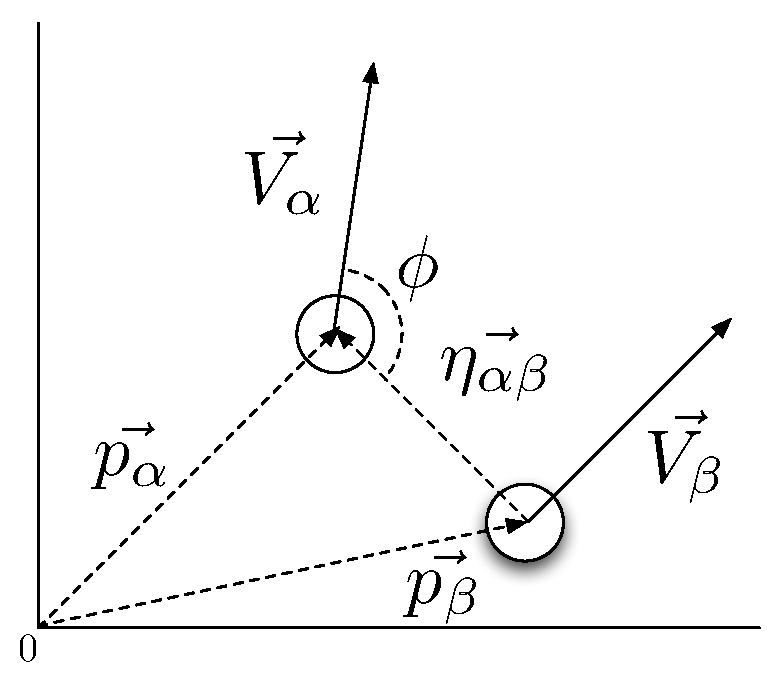
\includegraphics[scale=0.35]{Figures/NotationOfInteraction.pdf}} 
    \caption[Notation of the interaction between two agents]{Illustration of the notation for the interaction between agents.
	     An addition and difference to \ref{NotationOfWall} is that the wall has been replaced by pedestrian $\beta$.
	     $\eta_{\alpha \beta}$ is the normal vector pointing from $\alpha$ to $\beta$, and $\phi$ is the angle between $\alpha$'s 
	     velocity vector and $\beta$'s center of mass.}
    \label{NotationOfInteraction}
\end{figure}

Here $A_{\alpha}^{1}$, $A_{\alpha}^{2}$, $B_{\alpha}^{1}$, $B_{\alpha}^{2}$ 
and $\lambda_{\alpha}$ are all constants that can differ for each agent. 
$r_{\alpha \beta}$ is the sum of the radii of $\alpha$ and $\beta$ that is 
$r_{\alpha \beta} = r_{\alpha} + r_{\beta}$. $d_{\alpha \beta}$ is the 
distance from the center of mass of agent $\alpha$ and the center of mass of 
agent $\beta$ and is therefore given by $d_{\alpha \beta} = 
\|\vec{r_{\alpha}}\left( t \right) - \vec{r_{\beta}}\left( t \right) \|$.
$\eta_{\alpha \beta}$ is the normal vector pointing from $\alpha$ to $\beta$ 
and it is given by:

\begin{equation}
    \eta_{\alpha \beta} =
        \frac{\vec{r_{\alpha}}(t) - \vec{r_{\beta}}(t)}
             {\|\vec{r_{\alpha}}(t) - \vec{r_{\beta}}(t) \|}
\end{equation}

the angle $\phi$ in \eqref{agentinteraction} is the angle between the normal 
vector pointing from agent $\beta$ to $\alpha$ and the direction in which 
agent $\alpha$ is moving. Cosine to the angle is 

\begin{equation}
\cos \left( \phi \right)
	\left( t \right) 
		= 
	- \vec{\eta_{\alpha \beta}}
		\left( t \right) 
	\cdot 
\vec{e_{\alpha}}\left( t \right)
\end{equation}

Equation \eqref{agentinteraction} is divided into two terms. The first term on 
the right hand side reflects the agents tendency to stay at a certain distance 
from other agents. This part of the force is called the private sphere because 
the agent prefers to have some free space around him if possible. The radius 
of the private sphere can differ from agent to agent. The constant 
$A_{\alpha}^{1}$, $B_{\alpha}^{1}$ and $\lambda_{\alpha}$ control the nature 
of the private sphere $A_{\alpha}^1$ and $B_{\alpha}^1$ control the strength 
and range of the interaction respectively. $\lambda_{\alpha}$ is there to take 
into account a persons tendency to focus on things happening in front of him 
rather than behind him.	% we should make a drawing of this.

The second term of equation \eqref{agentinteraction} deals with physical interaction.
In the situation where the density of the crowd is high the agents will have be closer
to each other and the social sphere is undermined. % go more into detail here 
So if we look away from the social sphere for a minute and concentrate on the physical
interaction we will see that if we omit the social sphere the calculation will be reduced to
to:

\begin{equation}\label{re2}
\overrightarrow{f_{\alpha\beta}}(t) = A_{\alpha}^{2} exp\left[ \frac{r_{\alpha\beta} - d_{\alpha}\beta}{B_{\alpha}^{2}}\right]  \overrightarrow{n_{\alpha\beta}}
\end{equation}

Taking the norms of both sides of Equation (\ref{re2}), we can draw the relation between the value of $\overrightarrow{f_{\alpha\beta}}(t)$ and $ d_{\alpha\beta} $, as shown in Figure 
(\ref{fig:physicalinteraction1}).\\

\begin{figure}
    \centering
    {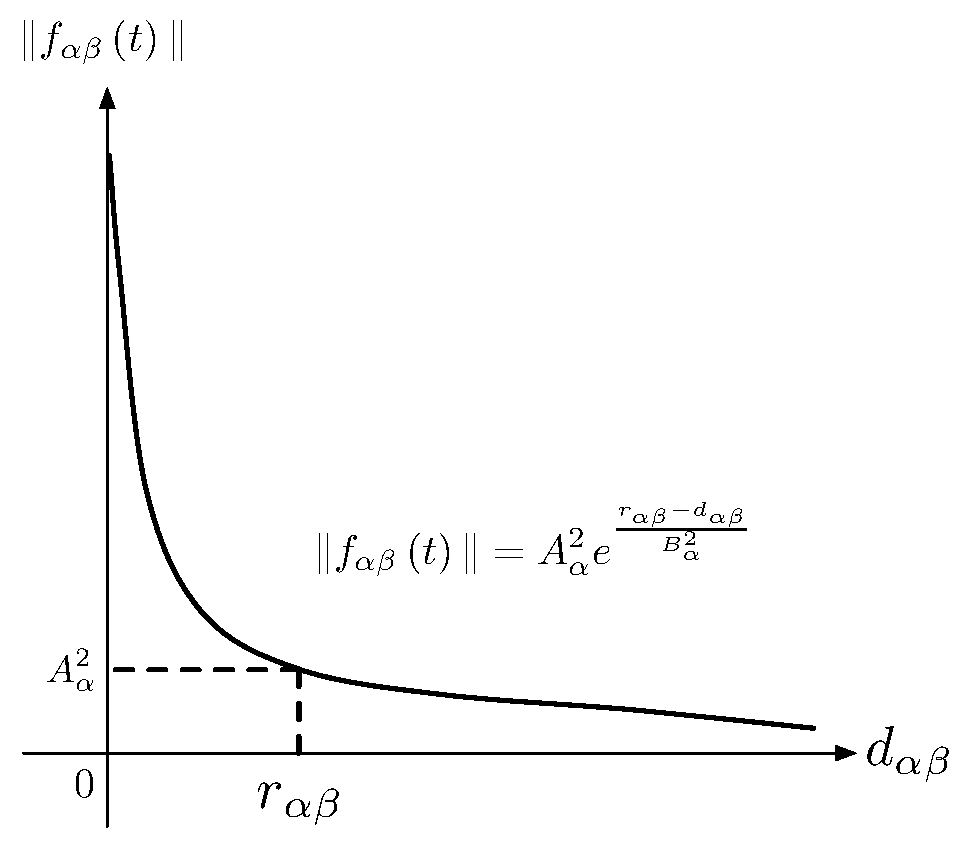
\includegraphics[scale=0.45]{Figures/physicalinteraction.pdf}} 
    \caption[Psysical interaction]{Illustration of the function about the interaction force 
        $f_{\alpha\beta}(t)$ and the distance between two agents
        $d_{\alpha \beta}$. It follows that the smaller the distance between two agents, the greater the interaction force is. }
    \label{fig:physicalinteraction1}
\end{figure}

There is one intersection of the graph and the  axis at:

\begin{equation}
	\left( d_{\alpha \beta} , \| \vec{f_{\alpha \beta}} \left( t \right) \| \right)
 =
	\left( 0 , A_{\alpha}^{2} exp\left( \frac{r_{\alpha\beta} }{B_{\alpha}^{2}}\right)  \right) 
\end{equation}

If put into the constants, we will be able to get a maximum value of $ f_{\alpha\beta}(t) $, 
since the distance between agents cannot be negative. Here we set $ A_{\alpha}^{2} = 3 m/s^{2} $, 
$ r_{\alpha\beta} = 0.6 m $, and $ B_{\alpha}^{2} = 0.2 m $, so 
$ f_{\alpha\beta}(t)^{max} \doteq 60 m/s^{2} $, which is about six times the gravitational 
acceleration and represents a rather large force between agents (as large as six person's weight).

%TODO: remember to finish this section

% TODO: again lets  have a little summation here. What kinds of dynamics does the
% social interaction part of the model yield. 


\subsection{Repulsion from other agents}
The third term on the right hand side of equation \eqref{model} is a summation of all the 
force between agent $\alpha$ and agent $\beta$. The equation we use is taken from a newer article \cite{ABconstant}. We did this because the original article contains two constants that is not given in the articel and in a mail we were adviced, by the authors, to use the values and equation from the new article. 

The function for the repulsion between pedestrians depends on the position vector and the velocity of 
both agents, and it is given by:

\begin{equation}
        \vec{f_{\alpha \beta }}\left( t \right) = w\left(\phi_{\alpha \beta}\right)\vec{g}\left(d_{\alpha \beta}(t)\right)
    \label{eq:agentinteraction}
\end{equation}

\begin{itemize}
\item $w\left(\phi_{\alpha \beta}\right)$ is a function of the angle between two pedestrians. It is given as: 

\begin{equation}
    w\left(\phi_{\alpha \beta}\right)=
    \left(
        \lambda_{\alpha} + \left(
            1 - \lambda_{\alpha}
        \right)
		\frac{1+\cos{\phi}}{2}
    \right) 
    \label{angleAB}
\end{equation}

the angle $\phi_{\alpha \beta}$ is the angle between the normal 
vector pointing from agent $\beta$ to $\alpha$ and the direction in which 
agent $\alpha$ is moving. Cosine to the angle is 

\begin{equation}
\cos \left( \phi \right)
	\left( t \right) 
		= 
	- \vec{\eta_{\alpha \beta}}
		\left( t \right) 
	\cdot 
\vec{e_{\alpha}}\left( t \right)
\end{equation}

$\lambda_{\alpha}$ is governing a persons tendency to focus on things happening in front of him 
rather than behind him. It will have a value  $0\leq \lambda_{\alpha}\leq 1$

\item A value of $\lambda_{\alpha}=1$ means that the force won't depent on the angle. Thus $\alpha$ will react the same to $\beta$ no matter if $\beta$ is in the front or comes from the side or back. A value of $0$ will on the other hand give the maximum angle depence. We find that $0\leq w\left(\phi_{\alpha \beta}\right)\leq1$ when $-1 \leq \cos \left( \phi \right) \left( t \right) \leq 1$. From this we see that $\alpha$ wont be affected at all if $\beta$ is coming from behind and the force will be maximum when $\beta$ comes directly in the front. It should be noted that in general one will find that the maximum of $w\left(\phi_{\alpha \beta}\right)$ always will be $1$ and the minimum will be equal to $\lambda_{\alpha}$.   

	% we should make a drawing of this.

\item The force, without the effect of $w\left(\phi_{\alpha \beta}\right)$, is given as the second term, in the right hand side of equation \ref{agentinteraction}. The function is:  
\begin{equation}
	\vec{g} 
	\left(
	d_{\alpha \beta}
	\right)
	=
	 A_{\alpha} e^{ \left(\frac{ r_{\alpha \beta} - d_{\alpha \beta}}{B_{\alpha}}\right)}
	\vec{n}_{\alpha \beta}
	        \label{re}	
\end{equation}

Here $A_{\alpha}$ and $B_{\alpha}$ are constants that can differ for each agent. 
$r_{\alpha \beta}$ is the sum of the radii of $\alpha$ and $\beta$ that is 
$r_{\alpha \beta} = r_{\alpha} + r_{\beta}$. $d_{\alpha \beta}$ is the 
distance from the center of mass of agent $\alpha$ and the center of mass of 
agent $\beta$ and is therefore given by $d_{\alpha \beta} = 
\|\vec{r_{\alpha}}\left( t \right) - \vec{r_{\beta}}\left( t \right) \|$.
$\eta_{\alpha \beta}$ is the normal vector pointing from $\alpha$ to $\beta$ 
and it is given by:

\begin{equation}
    \eta_{\alpha \beta} =
        \frac{\vec{r_{\alpha}}(t) - \vec{r_{\beta}}(t)}
             {\|\vec{r_{\alpha}}(t) - \vec{r_{\beta}}(t) \|}
\end{equation}

\begin{figure}[ht]
    \centering
    {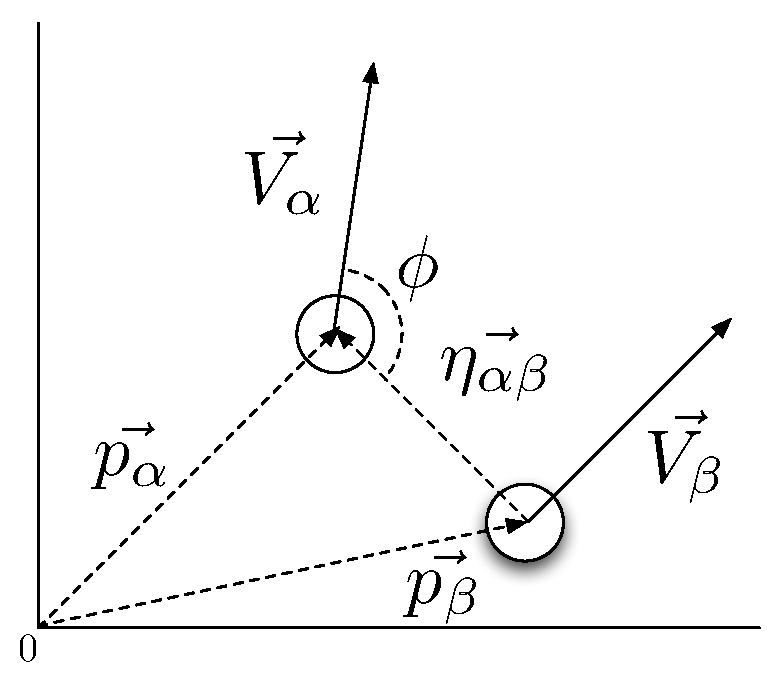
\includegraphics[scale=0.35]{Figures/NotationOfInteraction.pdf}} 
    \caption[Notation of the interaction between two agents]{Illustration of the notation for the interaction between agents.
	     An addition and difference to \ref{NotationOfWall} is that the wall has been replaced by pedestrian $\beta$.
	     $\eta_{\alpha \beta}$ is the normal vector pointing from $\alpha$ to $\beta$, and $\phi$ is the angle between $\alpha$'s 
	     velocity vector and $\beta$'s center of mass.}
    \label{fig:NotationOfInteraction}
\end{figure}


%Equation \ref{agentinteraction} is given by two terms. 
%The first term determines how much the the angle between the agents is and how much this angle should affect the force. 
%The constant $\lambda$ is the one controling the importance of the angle.
%The second term reflects the pedestrians tendency to stay at a certain distance 
%from other agents. The constants $A_{\alpha}$, $B_{\alpha}$ is the strength 
%and range of the interaction respectively and controls how big the force will be at a certain distance.  




\item Taking the norms of both sides of Equation (\ref{re}), we can draw the relation between the value of $\overrightarrow{f_{\alpha\beta}}(t)$ and $ d_{\alpha\beta} $, as shown in Figure 
(\ref{fig:physicalinteraction2}).\\

\begin{figure}
    \centering
    {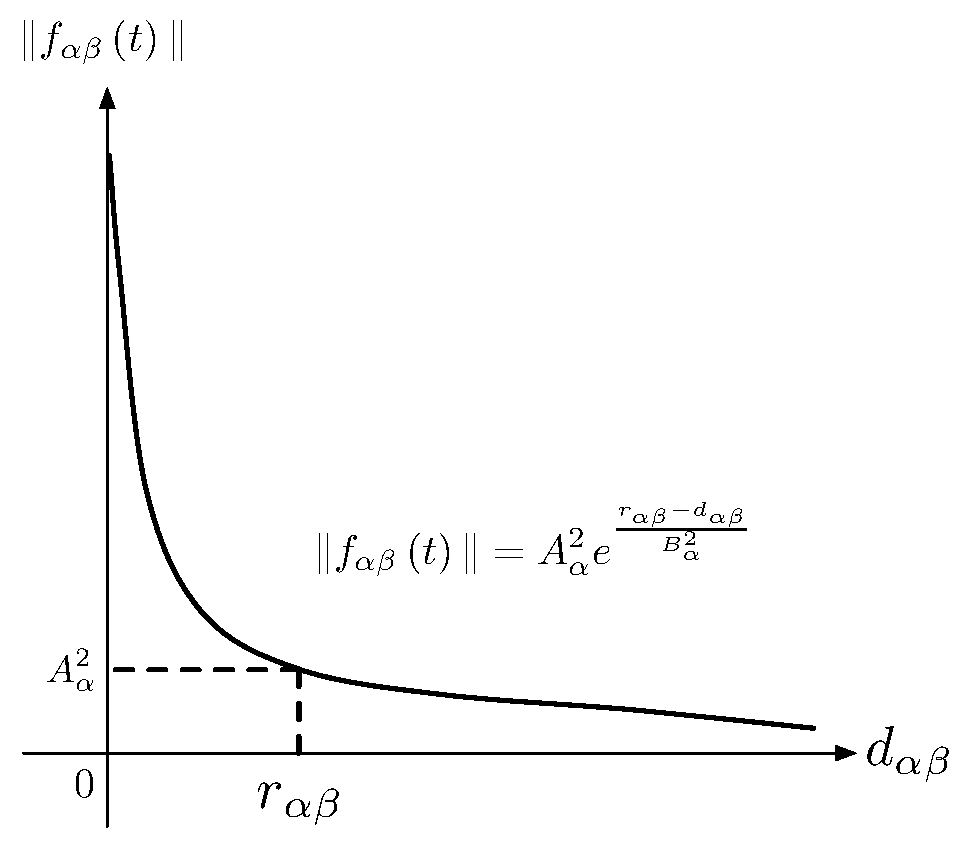
\includegraphics[scale=0.45]{Figures/physicalinteraction.pdf}} 
    \caption[Psysical interaction]{Illustration of the function about the interaction force 
        $f_{\alpha\beta}(t)$ and the distance between two agents
        $d_{\alpha \beta}$. It follows that the smaller the distance between two agents, the greater the interaction force is. }
    \label{fig:physicalinteraction2}
\end{figure}

There is one intersection of the graph and the  axis at:

\begin{equation}
	\left( d_{\alpha \beta} , \| \vec{f_{\alpha \beta}} \left( t \right) \| \right)
 =
	\left( 0 , A_{\alpha} exp\left( \frac{r_{\alpha\beta} }{B_{\alpha}}\right)  \right) 
\end{equation}

\item If we put in values for the constants, we will be able to get a maximum value of $ f_{\alpha\beta}(t) $, 
since the distance between agents cannot be negative. Here we take values from \cite{ABconstant} $ A_{\alpha} = 0.42 m/s^{2} $, 
$ r_{\alpha\beta} = 0.6 m $, and $ B_{\alpha} = 1.65 m $, so 
$ f_{\alpha\beta}(t)^{max} < 0.64 m/s^{2} $. It can never be exactly $0.64m/s^2$ since the normal vector will be undefined when two pedestrians are in the exact same spot.

\end{itemize}

%TODO: remember to finish this section

%TODO: again lets  have a little summation here. What kinds of dynamics does the
% social interaction part of the model yield.

\subsection{The attractive forces between some agents}
The fourth and last term in \eqref{model} represents the force from attraction 
in the room. Attractions can be either be either interesting sculptures or 
sights or familiar persons the agent prefer to be close to, such as friends 
and family. The mathematical structure of this force is the same as the force 
from other agents, however it is opposite in algebraic sign and has different 
constants. 

To get an overview of how the model is put together look a figure \ref{overview}
with the aid of table \ref{tableofconstandvar}

\begin{figure}[hb] %with some more comments i think that this figure could serve as a summation of the entire section
    \centering
    {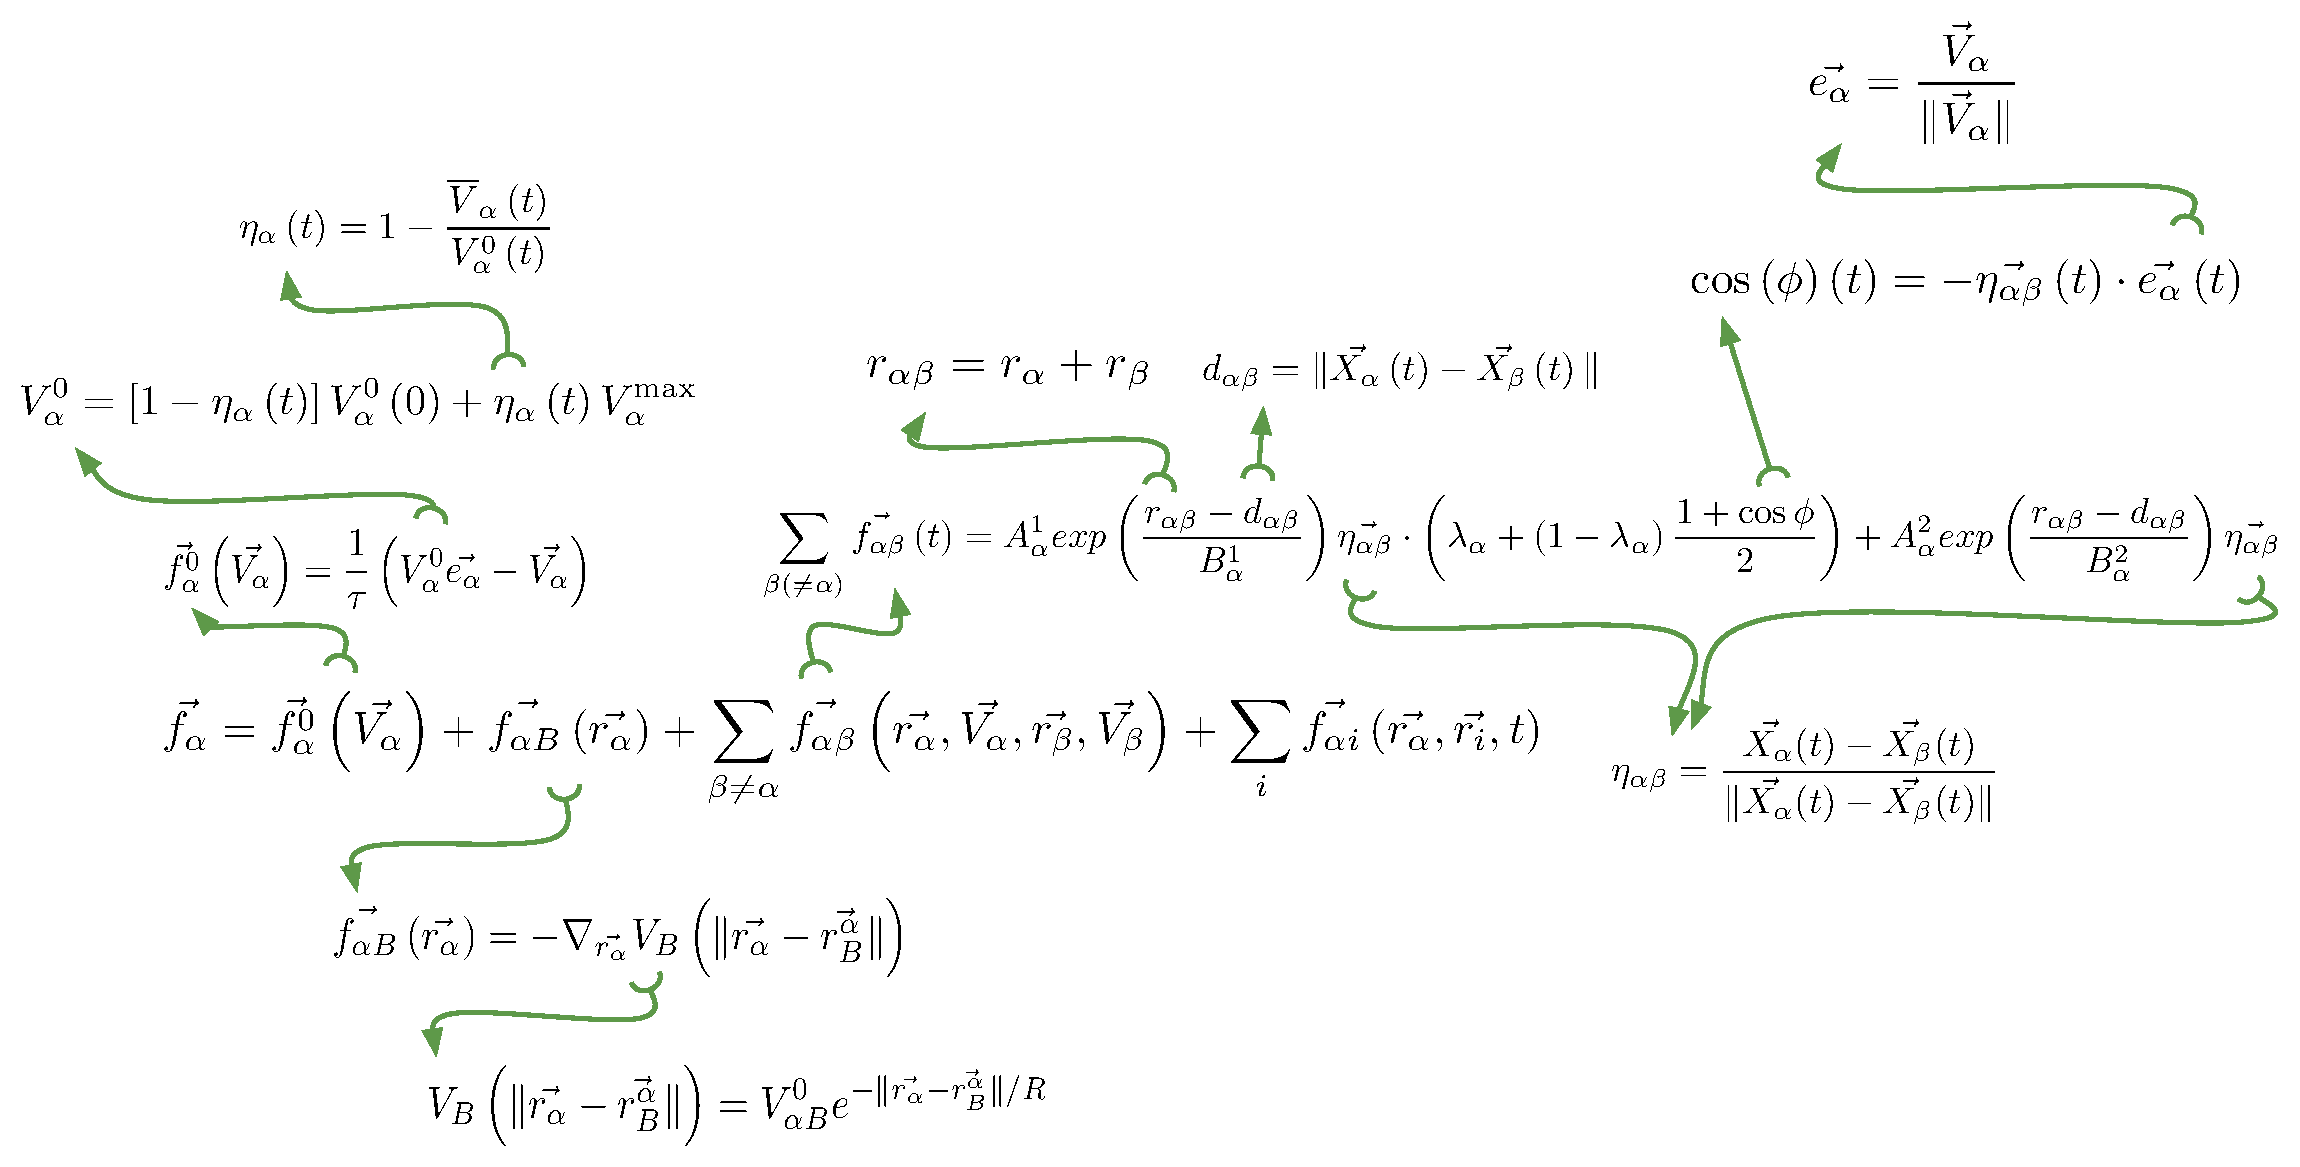
\includegraphics[scale=0.45]{Figures/overview.pdf}} 
    \caption[Overview of the model]{Illustration of an overview of how the model is put together. The different equations and their notation is written to give the 
	     reader an overview of how the model looks like.}
    \label{overview}
\end{figure}
